\chapter{Implementation}

% TODO - DATES
\section{Pre-Development} 
Before starting the project it was important to ensure the foundations were in place for creating it. 

\section{Sprint 1: 26th May - 15th June}
The main focus of this sprint was to create the basic infrastructure for the project. As established during the planning phase, the intention was to create a Blazor web application using a server-client architecture, a model shown in Figure \ref{fig:static-server-client-model}. This utilises two main features:

\begin{itemize}
    \item Server: A backend server that handles more computationally intensive operations. Can be interacted with only by the client, typically through HTTP requests.
    \item Client: The web application the user sees. Designed to be fast and lightweight, it can handle small scale computation on the user's local machine, but requests more intensive work from the server.
\end{itemize}

By handling intensive actions such as retrieving data from the third-party API on the backend server, the operations can run without causing the front-end to deadlock. This can often be seen when websites freeze while operations are running - they run on the thread that is handling displaying the user interface, and the computer cannot do both at the same time. 

\begin{figure}
    \centering
    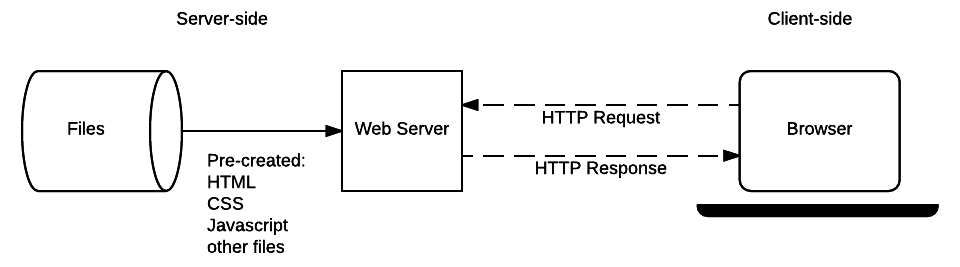
\includegraphics[width=1\linewidth]{Figures/basic_static_app_server.png}
    \caption{Basic Server Client Model for Web Applications \cite{client-server-model-graphic}}
    \label{fig:static-server-client-model}
\end{figure}

\subsection{Moving From FastF1 to OpenF1}
Lorem Ipsum

\section{Sprint 2: 16th June - 6th July}

\subsection{Move to WPF}

During the previous sprint, it became clear that completing a satisfactory piece of software in the intended format - particularly an HTML, CSS, and JavaScript front-end - would not be possible within the intended timeframe. Developing this to the required standard would require a degree of proficiency that could not be achieved to the necessary standards within the project's constraints, and attempting to learn the technologies alongside developing the undercut analysis tool would introduce significant risk to delivering a complete and functional tool to the required level. 

In light of this, it was decided to modify the project to be a stand-alone software tool. This would be a Windows Presentation Foundation (WPF) desktop application. In this context, WPF provided several advantages:

\begin{itemize}
    \item It leverages pre-existing knowledge for the developer, significantly reducing the learning curve and allowing all time spent on the project to be focused on functionality.
    \item The framework offers built-in Graphical User Interface (GUI) tools, including data binding, allowing simple front-end development that can adapt to user choices, such as changing events.
    \item WPF allows rapid prototyping and testing without requiring the complexities of in-browser development. This was a significant improvement, as numerous problems had occurred while trying to debug problems in the Blazor app, including being unable to add breakpoints to the code for step-through debugging, as well as the development infrastructure acting inconsistently when being used on different machines. WPF is native to Windows, so is much more consistent and links directly to a development environment for debugging.
\end{itemize}



\section{Sprint 3: 7th July - 27th July}
\subsection{API Reliability}
Lorem Ipsum

\section{Sprint 4: 28th July - 17th August}
Lorem Ipsum

\section{Sprint 5: 18th August - 7th September}
Lorem Ipsum

% SHORT
\section{Sprint 6: 8th September - 21 September}
Lorem Ipsum